V předchozí kapitole jsme se seznámili s technickými principy a postupy, které se uplatňují v BigData konceptu. V této kapitole se budu zabývat jedním z hlavních témat práce a tím je open source řešení pro platformu BigData od organizace Apache Foundation, také známý jako Apache Big Data Stack. Tento stack se skládá z několika aplikací, které (až na jednu výjimku) na sobě nejsou nikterak závislé. V závěru této kapitoly se budu rovněž důkladně věnovat pro nás nejdůležitější části tohoto stacku, kterou je NoSQL databázový systém Cassandra.

\section{Hadoop}




Hadoop je softwarová knihovna napsaná v programovacím jazyce Java, která umožňuje distribuované zpracování velkého množství dat napříč clusterem pomocí jednoduchých programovacích modelů. Hadoop je navržený tak, aby dobře škáloval cluster tvořící jeden až několik tisíc počítačů, kde každý nabízí lokální výpočetní výkon a úložiště dat. Hadoop řeší problémy s hardwarem na aplikační vrstvě, díky čemuž je možné navrhovat vysoce dostupné služby na clusteru počítačů, aniž bychom se museli strachovat výpadků. 4 základní komponenty Hadoopu tvoří nejpodstatnější část pro celou analytickou práci s daty. Všechny ostatní aplikace přímo či nepřímo některé části Hadoopu používají nebo jsou na nich dokonce založeny. Jaké tedy jsou tyto 4 komponenty Hadoopu?


\begin{figure}[h]
\centering

\includegraphics[scale=0.15]{images/hadoop}
\caption{Logo Apache hadoop}
\label{fig:yarn}

\end{figure}


\subsection{Hadoop Commons}
Jedná se pouze o základní sadu nástrojů podporující a propojující ostatní moduly Hadoopu.


\subsection{Hadoop File System (HDFS)}
Open source distribuovaný filesystém, jehož některé prvky vychází z dříve zmíněného GFS. HDFS umožňuje uložit velké množství dat mezi jednotlivé uzly. HDFS nabízí velice dobré škálování s rostoucím objemem dat. Ostatní technologie z Apache Big Data Stacku filesystém využívají ke sběru a ukládání výsledků jejich analytických procesů. HDFS cluster se skládá primárně z NameNode, který řídí filesystémová metadata a z DataNodů, které data uchovávají. 

\subsection{Hadoop MapReduce}
MapReduce jsme zmínili výše a tak zde jen zopakuji, že se jedná o programovací paradigma a framework na paralelní zpracování dat. Nabízí API, díky kterému můžeme jednoduše programovat vlastní MapReduce operace. Tento framework nabízí základní kostru, kterou programátor doplní a o vše ostatní se pak již postará samotná knihovna. Přesto však veškerá logika programu závisí na programátorovi. 

\subsection{Hadoop YARN}
Tento modul se stará o plánování jednotlivých MapReduce programů a o správu dostupných zdrojů v celém clusteru. Také rozhoduje o tom, jaká data se kam budou posílat a počítat. Základní myšlenkou architektury YARNu je mít jeden globální uzel, který se nazývá \uv{Resource Manager} a pro každý běh aplikace mít tzv. \uv{Application Master}, který má na starosti komunikaci s \uv{Node Managery} a dohlížení na spouštění jednotlivých Tasků. Resource Manager se skládá ze 2 hlavních komponent – Plánovače a Aplikačního manažera. Plánovač je zodpovědný za alokování zdrojů pro běžící aplikace. Aplikační manažer je zodpovědný za příjem nových MapReduce programů a jejich správné zařazení. NodeManager je agent běžící na každém stroji, který je zodpovědný za aplikační kontejnery, monitoruje stav dostupných prostředků stroje a ohlašuje se Resource Manageru, který tak má potřebné informace k přerozdělování nových úkolů.

\begin{figure}[h]
\centering
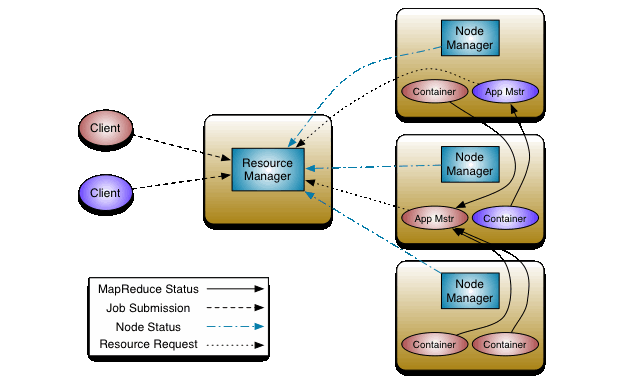
\includegraphics[scale=0.7]{images/yarn_architecture}
\caption{Architektura Hadoop YARN}
\label{fig:yarn}

\end{figure}



\newpage 

\section{HBase}
HBase je NoSQL databázový systém, který je založený na principu Google BigTable. Jedná se o druhou nejpoužívanější NoSQL databázi v Apache Big Data Stacku. Implementačně je závislá na HDFS, který používá k ukládání dat. Výhodou je velice jednoduchá a rychlá integrace s Hadoop MapReduce. HBase zdědil po Hadoopu také jeho Master-Slave architekturu.


\section{Hive}


Apache Hive je data warehouse infrastruktura postavená na vrchu Hadoopu pro poskytování analýzy a dotazování se nad daty. Původně byl tento software vyvinut ve společnosti Facebook, nyní se o jeho rozvoj starají společnosti, jako je NetFlix a Amazon. Hive podporuje analýzu velkých datasetů uložených v HDFS nebo HDFS-kompatibilních systémech, jako je například CassandraFS nebo Amazon S3. Syntaxe jeho dotazovacího jazyka HiveQL je velice podobná SQL, a proto ho mohou inženýři ovládající tento jazyk velice brzy ovládnout. HiveQL nabízí programátorům prostředky, které nejsou běžně v NoSQL databázích dostupné (například funkce JOIN). 

\begin{wrapfigure}{r}{0.5\textwidth}
  \centering
    
\includegraphics[scale=0.5]{images/hive_logo}
\caption{Logo Apache Hive}

\end{wrapfigure}

Princip Hivu leží v převodu dotazu do kódu kompatibilního s Hadoop Mapreduce a následném spuštění výsledného programu na Hadoop clusteru. Obrovskou výhodou je, že programátor dostává v podstatě s nulovým snažením hotový MapReduce program, který by jinak musel zdlouhavě psát, což výrazně zvyšuje efektivitu tohoto programátora. Hive si standardně ukládá metadata do embedované databáze Derby. Podporuje pokročilejší funkce, jako jsou například indexy, kompresi nebo uživatelem definované funkce (UDF). Samozřejmostí jsou standardní matematické a řetězcové funkce aplikovatelné v HiveQL dotazech. 



\section{Pig}


Pig funguje na stejném principu jako Hive. Tedy, že převede vámi napsaný kód do hotového MapReduce řešení a tento kód spustí nad Hadoop clusterem. Tato knihovna byla napsána ve firmě Yahoo a později opensourcována pod Apache Foundation. Pig používá svůj vlastní jazyk pojmenovaný Pig Latin a oproti HiveQL nemá s SQL moc společných rysů. Latin se spíše podobá funkcionálním jazykům. Pig a Hive dělají tedy stejné věci, tak proč používat obojí? Je to spíše volba osobních preferencí či preferencí vašeho vývojářského týmu. S oběma technologiemi lze dosáhnout stejných výsledků. Přesto má Pig lepší uplatnění v případě tvorby komplikovanějších data flow a HiveQL se více hodí pokud jsou potřeba spíše ad-hoc dotazy. Přestože lze dosáhnout stejných výsledků s oběma platformami, určitě doporučuji umět obě a použít Hive nebo Pig v konkrétních situacích, kde má ta která platforma lepší užití. 



\section{SolR}

SolR [Solar] je vyhledávací platformou odvozenou od Apache Lucene. Mezi její hlavní výhody patří:

\begin{itemize}
\item Pokročilý full-text vyhledávací engine
\item Optimalizace pro vysokoobjemový tok dat
\item Otevřené rozhraní pomocí XML, JSON nebo HTTP
\item Lineární škálovatelnost, automatická replikace indexu, auto failover a samoobnovení
\item Indexace v téměř reálném čase
\item Možnost doprogramování vlastních pluginů
\end{itemize}

SolR využívá Lucene index, což znamená, že je formát striktně definovaný. Změna ve formátu indexu znamená reindexaci celého dokumentu. Díky snadnému nastavení, možnostem výstupu a pokročilým funkcím jako je například GeoSpatial, vyhledávání nebo facetové full text hledání je SolR v komerční a open source sféře vyhledávacím enginem číslo 1.


\section{Squoop}

Tento nástroj je velice užitečný, protože ne vždy chceme mít všechna data pouze v NoSQL databázích a pokud je to možné, využití výhod relačních databází je logickou volbou. Apache Squoop je nástroj pro hromadnou migraci z HDFS či kompatibilního filesystému do strukturovaných úložišť, jakými jsou právě například relační databáze. Přesun dat je navržený obousměrně, stejně tak můžeme využít Squoop k migraci dat z relačních databází do HDFS a kompatibilních systémů. Výhodou je vysoká efektivita a nízká časová investice oproti psaní vlastních migračních skriptů.

\section{Mahout}

Mahout je slovo, které pochází z hindštiny a jeho překladem do češtiny získáme slovní spojení „jezdec na slonovi“. Slonem se v BigData komunitě myslí projekt Apache Hadoop, který má slona ve svém logu a je právě s tímto zvířetem neodmyslitelně spojený. Projekt Mahout už svým názvem naznačuje využívání Hadoopu k vytvoření knihovny pro podporu škálovatelného \uv{Machine learningu}. Mahout je sada funkcí a algoritmů využívaných v odvětví machine learningu, naprogramovaných pomocí Hadoop MapReduce paradigmatu. Mahout se primárně zaměřuje na odvětví kolaborativního filtrování, clusterování a klasifikace dat. Mahout rovněž obsahuje vysoké množství matematických funkcí a algoritmů z oblasti lineární algebry a statistiky. V současné době lze Mahout využít na tyto základní způsoby užití. Doporučovací funkce na základě uživatelského chování, rozřazování dokumentů do clusterů na základě shody v obsahu a klasifikace dokumentů na základě již uložených kategorizovaných dokumentů. % seznam?

\section {ZooKeeper}

Autoři projektů v rámci Apache Foundation, a především ti zaměření na projekty BigData Stacku, mají pro metafory a různá symbolická spojení velkou slabost. Velká část projektů má v názvu nebo v logu nějaké zvíře, či alespoň referenci na něj. Ovšem uhlídat a spravovat byť malý, ale distribuovaný systém, může být velmi náročné a proto je potřeba ten správný hlídač. ZooKeeper (v překladu „hlídač ZOO“) je nástroj pro správu a konfiguraci distribuovaných systémů z platformy Apache BigData. 

